% 建议使用 XeLaTeX 或 LuaLaTeX 编译(中文与公式支持更佳)
\documentclass[UTF8,zihao=-4]{ctexart}

% 版式与常用宏包
\usepackage[a4paper,margin=2.5cm]{geometry}
\usepackage{amsmath, amssymb, amsthm}
\usepackage{bm}
\usepackage{hyperref}
\usepackage{graphicx}
\usepackage{caption}
\usepackage{float} % 强制图表位置 [H]
\usepackage{placeins} % 控制浮动体不跨越屏障
\usepackage{listings}
\usepackage{xcolor}
\graphicspath{{figures/}}

% 代码样式(与前序章节一致)
\lstdefinestyle{code}{
  basicstyle=\ttfamily\small,
  numbers=left,
  numberstyle=\tiny,
  numbersep=8pt,
  keywordstyle=\color{blue},
  commentstyle=\color{teal!70!black},
  stringstyle=\color{orange!70!black},
  showstringspaces=false,
  breaklines=true,
  frame=single,
  framerule=0.3pt,
  rulecolor=\color{black!15}
}
\lstset{style=code}

\title{逻辑回归(Logistic Regression):原理、公式、应用与实战}
\author{}
\date{\today}

\begin{document}
\maketitle
\tableofcontents

\section{引言}
逻辑回归通过 S 形函数(sigmoid)将线性组合的输出映射到 $[0,1]$,从而建模类别为 1 的条件概率。它具有良好的可解释性与概率输出,常用于风险评估、医疗诊断、CTR 预测等任务。

\section{原理与公式}
设 $\bm{x}\in\mathbb{R}^d,\ y\in\{0,1\}$,模型为:
\begin{equation}
  p(y=1\mid \bm{x}) = \sigma(z),\quad z = w_0 + \bm{w}^\top \bm{x},\quad \sigma(t) = \frac{1}{1+e^{-t}}.
\end{equation}
对数几率(logit)线性:$\log \tfrac{p}{1-p} = w_0 + \bm{w}^\top \bm{x}$。

给定样本 $\{(\bm{x}_i,y_i)\}_{i=1}^n$,二元交叉熵(负对数似然)为:
\begin{equation}
  \mathcal{L}(\bm{w},w_0) = -\sum_{i=1}^n \big[y_i\log p_i + (1-y_i)\log (1-p_i)\big],\quad p_i=\sigma(w_0+\bm{w}^\top\bm{x}_i).
\end{equation}
梯度:
\begin{equation}
  \nabla_{\bm{w}}\,\mathcal{L} = \sum_{i=1}^n (p_i - y_i)\,\bm{x}_i,\qquad \frac{\partial\mathcal{L}}{\partial w_0} = \sum_{i=1}^n (p_i - y_i).
\end{equation}
加入 $\ell_2$ 正则可缓解过拟合:$\tfrac{\lambda}{2}\lVert\bm{w}\rVert^2$;$\ell_1$ 则有助于稀疏化与特征选择。

阈值取 $0.5$ 时的判别边界满足 $\sigma(z)=0.5\iff z=0$,即超平面 $w_0+\bm{w}^\top\bm{x}=0$。

\section{应用场景与要点}
\begin{itemize}
  \item \textbf{特征缩放}:有助于优化收敛与系数可解释性;
  \item \textbf{类别不平衡}:可调阈值、设定类权重或重采样;
  \item \textbf{正则化}:$\ell_2$ 稳定系数,$\ell_1$ 促稀疏,缓解多重共线性;
  \item \textbf{概率输出}:便于排序与代价敏感决策;
  \item \textbf{系数解释}:关注胜算比 $e^{w_j}$ 的含义。
\end{itemize}

\section{Python 实战}
运行配套脚本以生成本章使用的图片。脚本仅依赖 NumPy 与 Matplotlib,并内置简易的逻辑回归实现,避免版本兼容问题。

\lstinputlisting[language=Python,caption={gen\_logistic\_regression\_figures.py}]{gen_logistic_regression_figures.py}

\section{运行效果}
核心插图如下所示。

\begin{figure}[H]
  \centering
  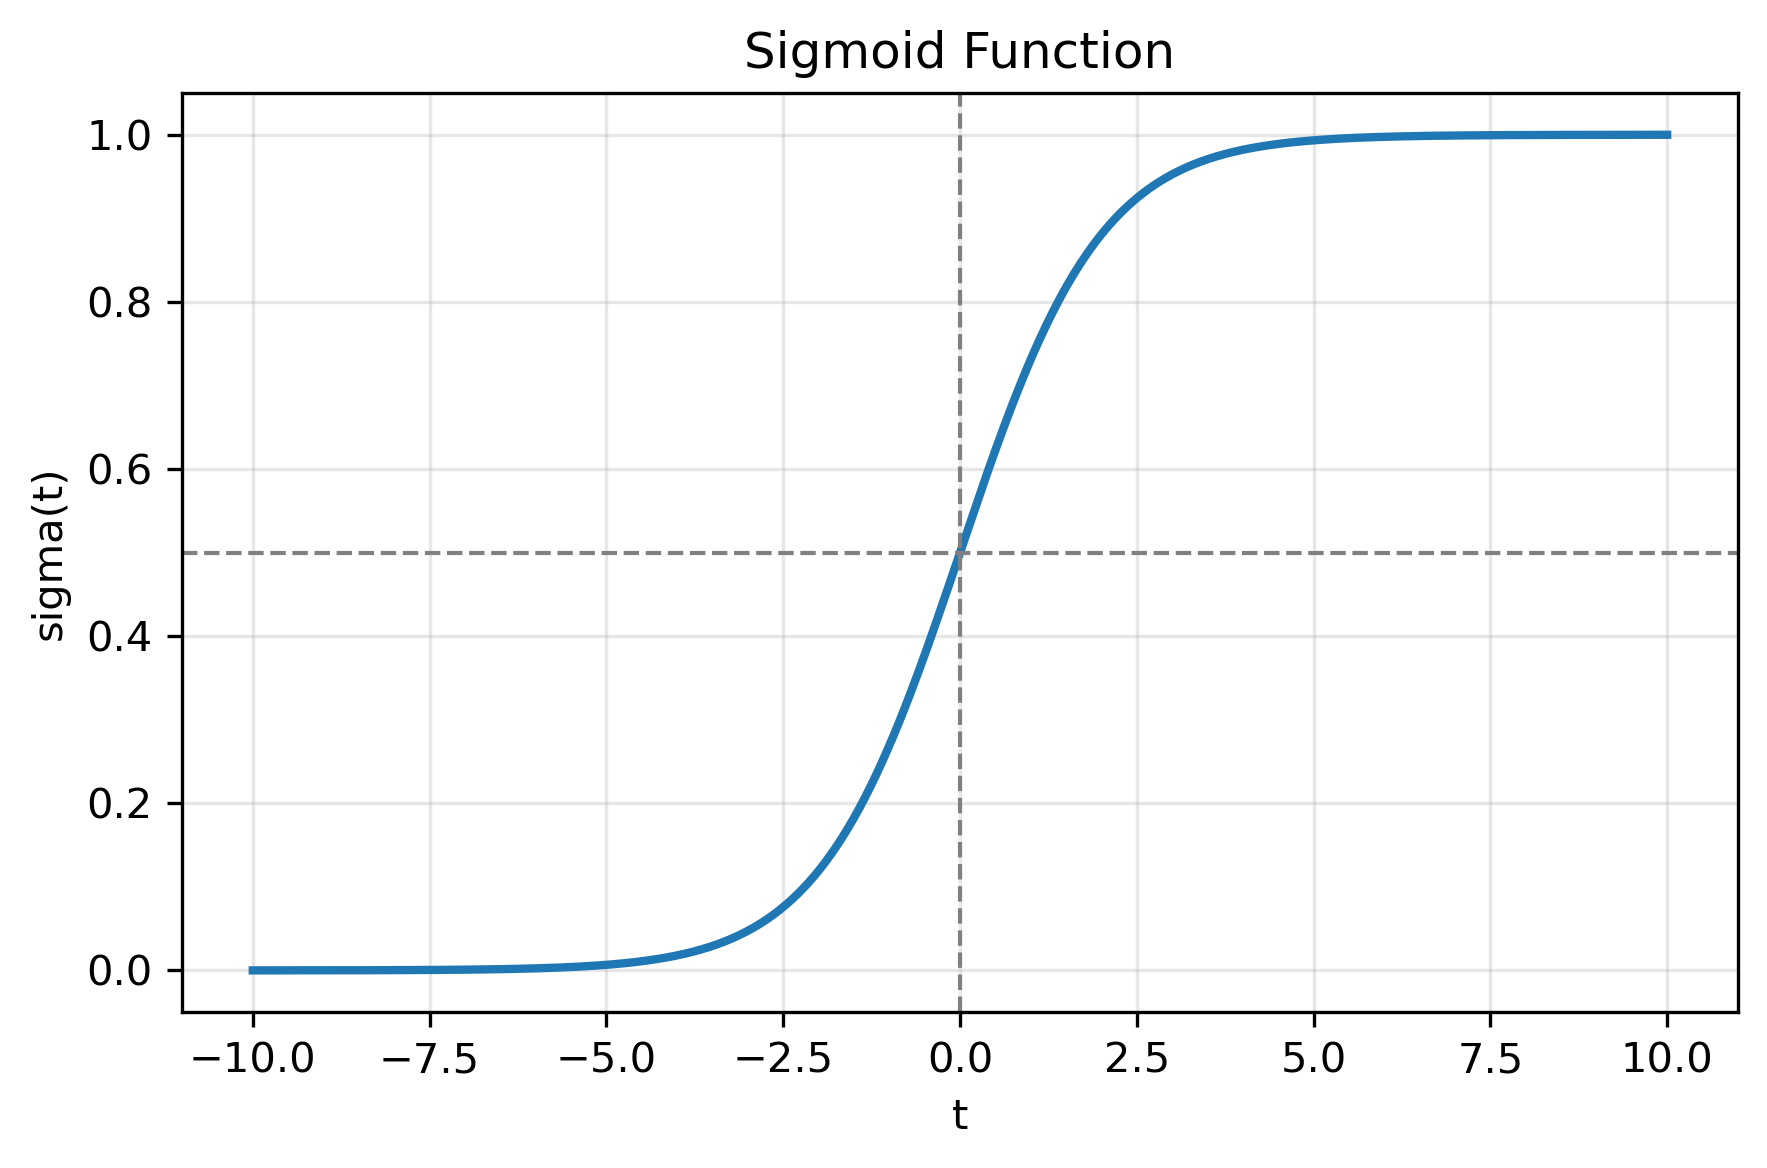
\includegraphics[width=0.65\linewidth]{sigmoid_curve.png}
  \caption{S 形函数 $\sigma(t)=1/(1+e^{-t})$}
  \label{fig:sigmoid}
\end{figure}

\begin{figure}[H]
  \centering
  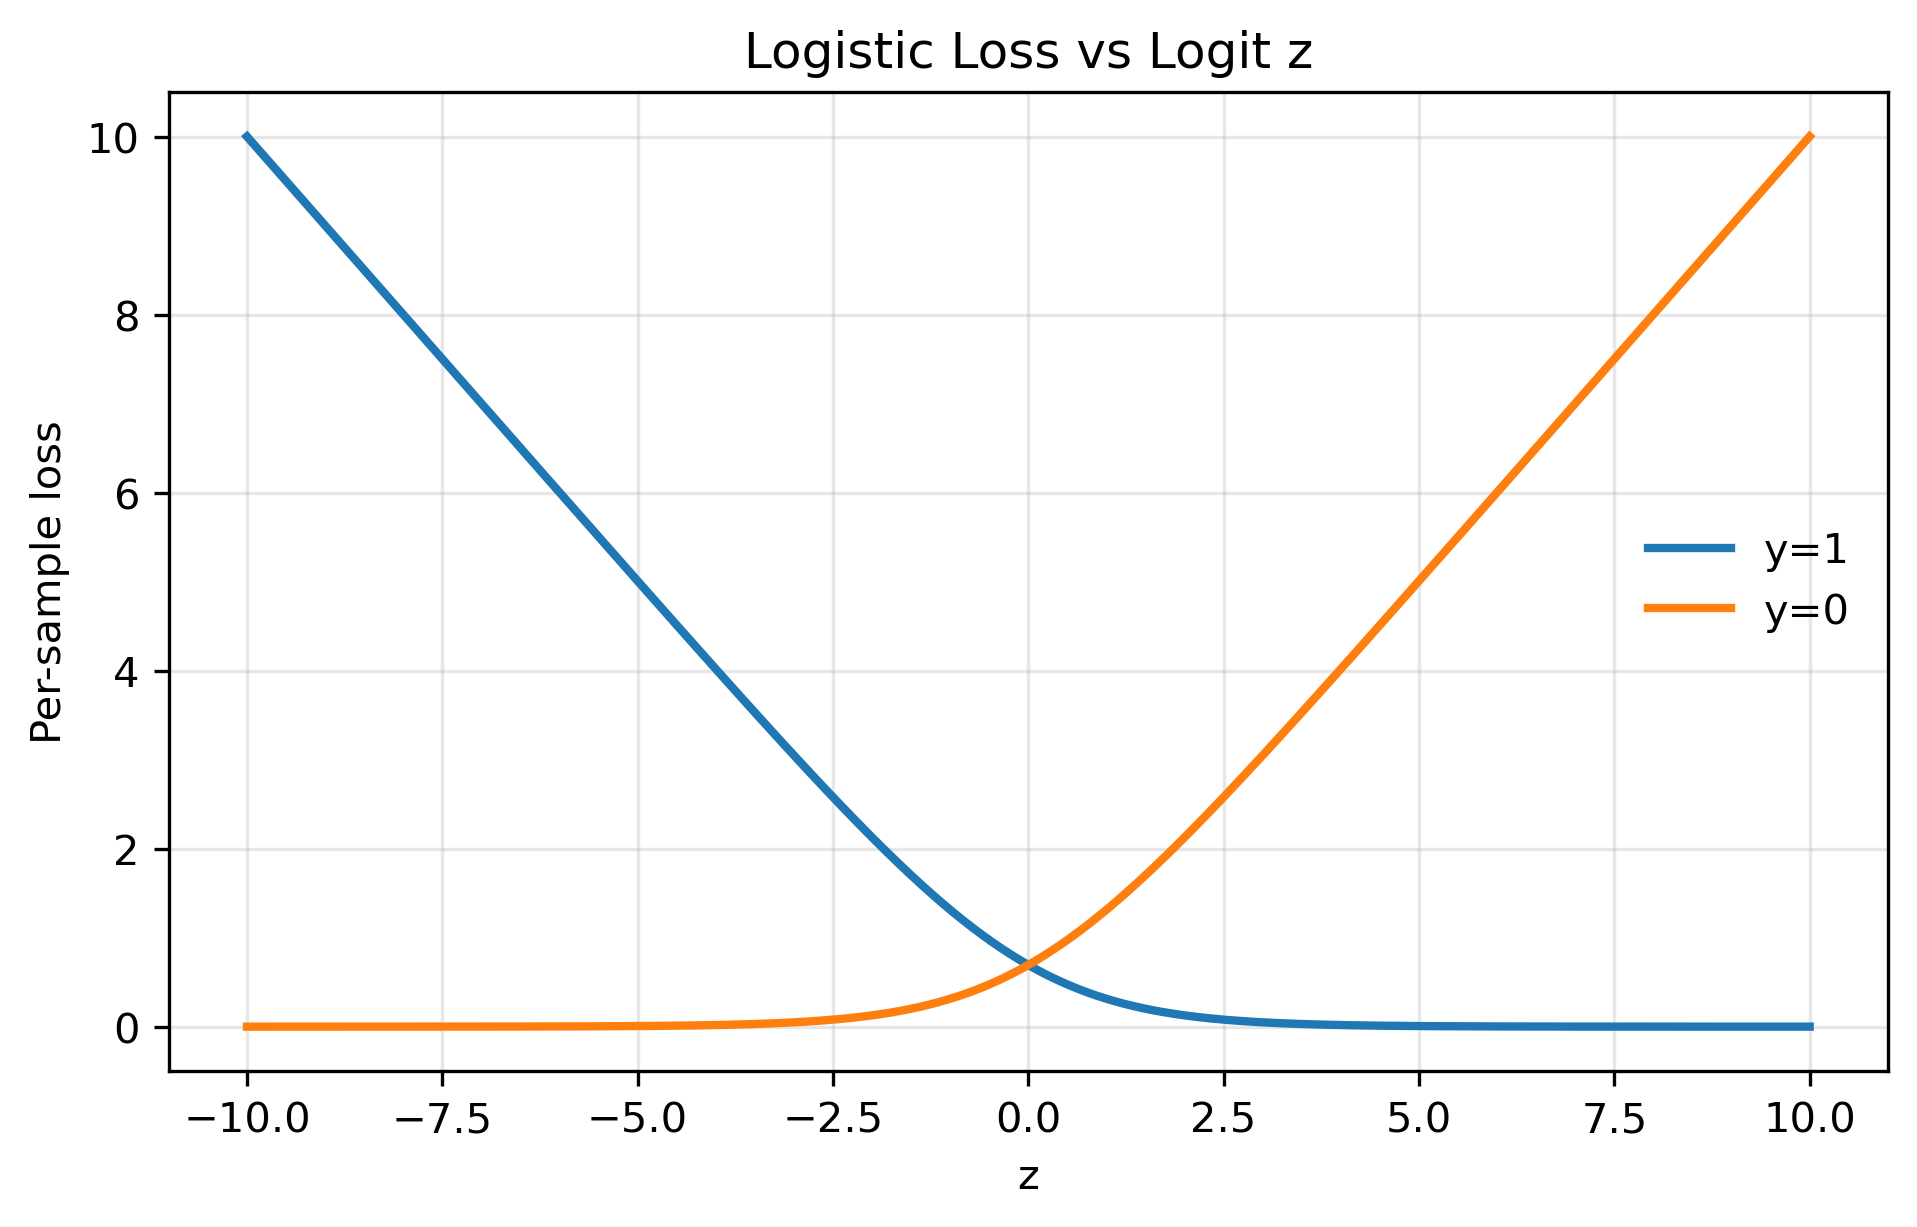
\includegraphics[width=0.7\linewidth]{logistic_loss_curves.png}
  \caption{单样本二元交叉熵随对数几率 $z$ 的变化曲线($y=0$ 与 $y=1$)}
  \label{fig:loss}
\end{figure}

\begin{figure}[H]
  \centering
  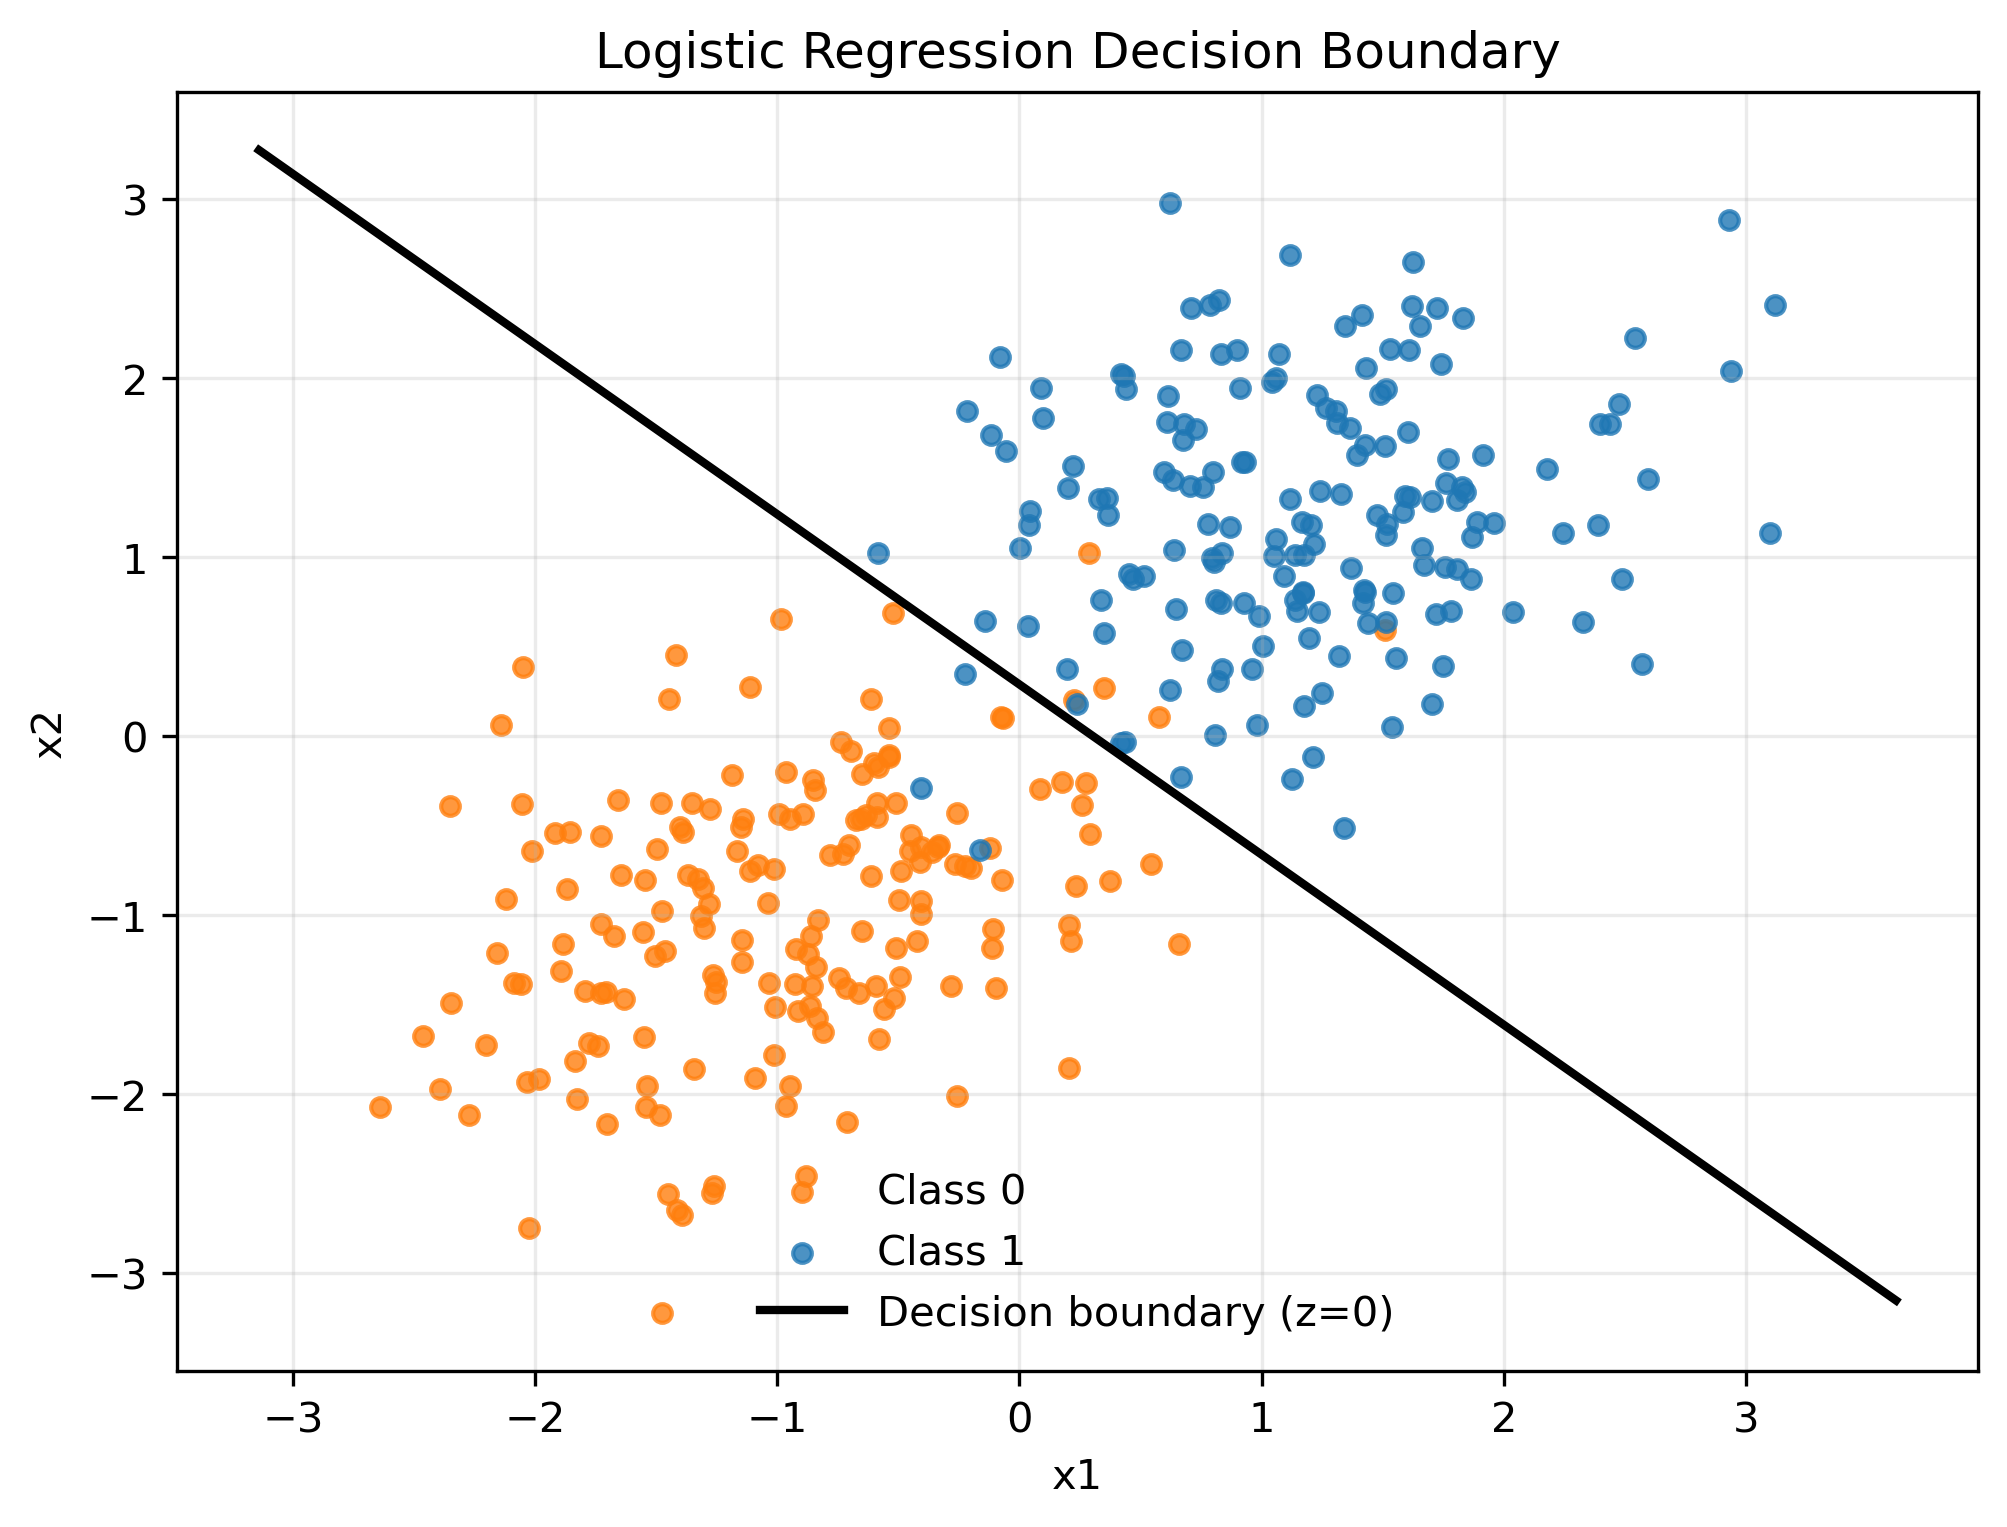
\includegraphics[width=0.78\linewidth]{decision_boundary.png}
  \caption{二维合成数据与学习到的逻辑回归判别边界}
  \label{fig:boundary}
\end{figure}

\begin{figure}[H]
  \centering
  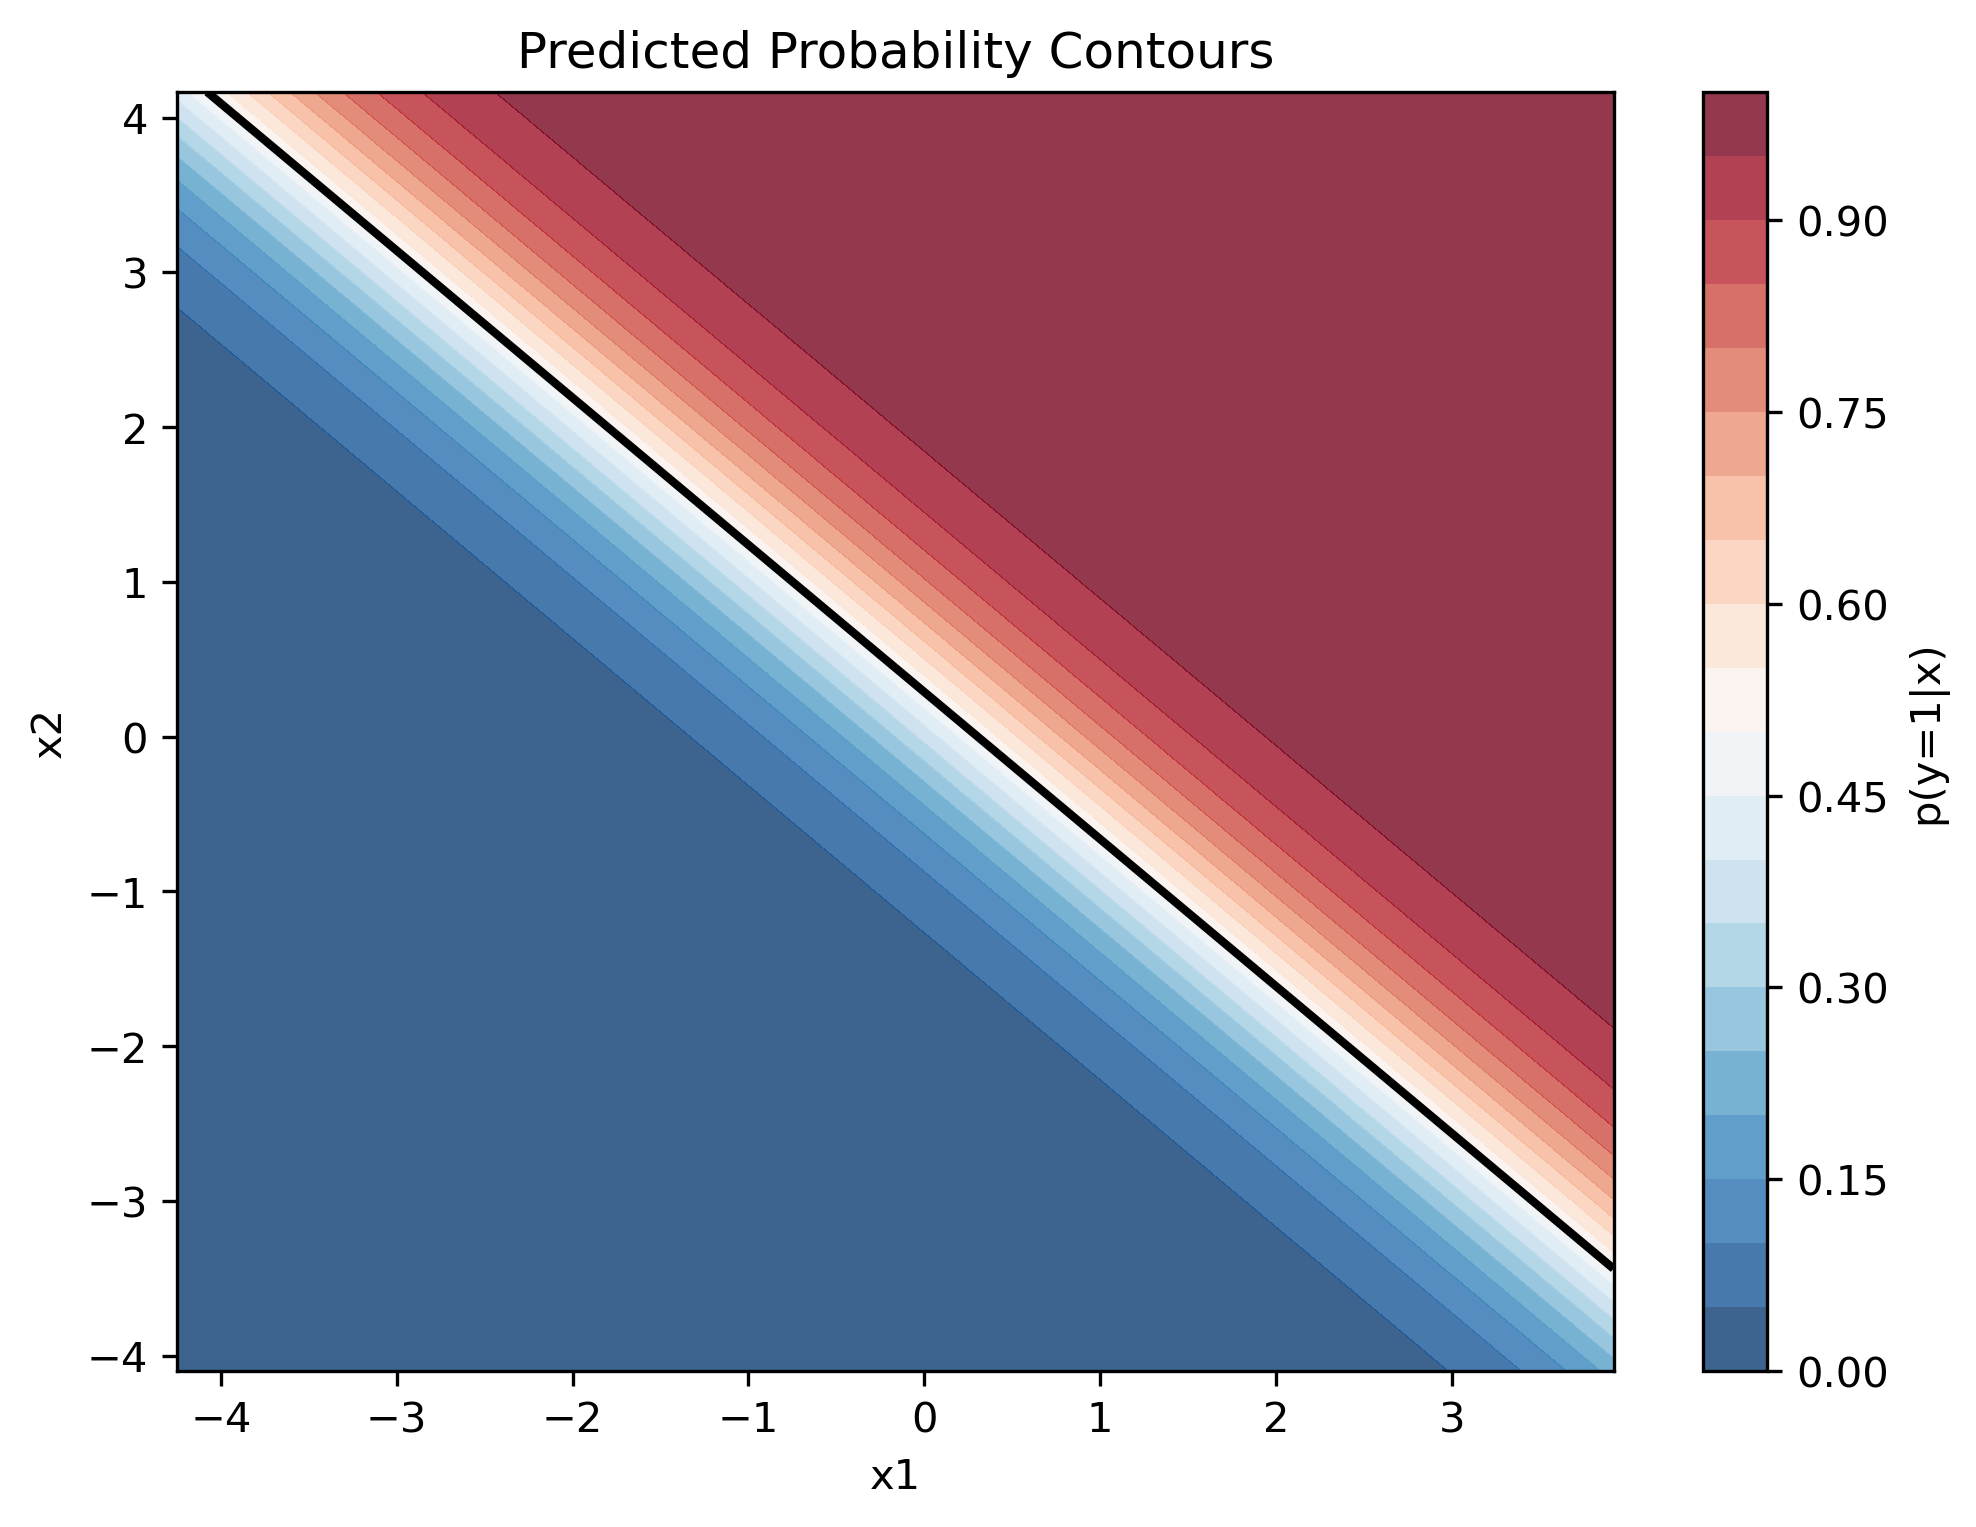
\includegraphics[width=0.78\linewidth]{probability_contours.png}
  \caption{网格上的预测概率等高线 $p(y=1\mid \bm{x})$}
  \label{fig:contours}
\end{figure}

\begin{figure}[H]
  \centering
  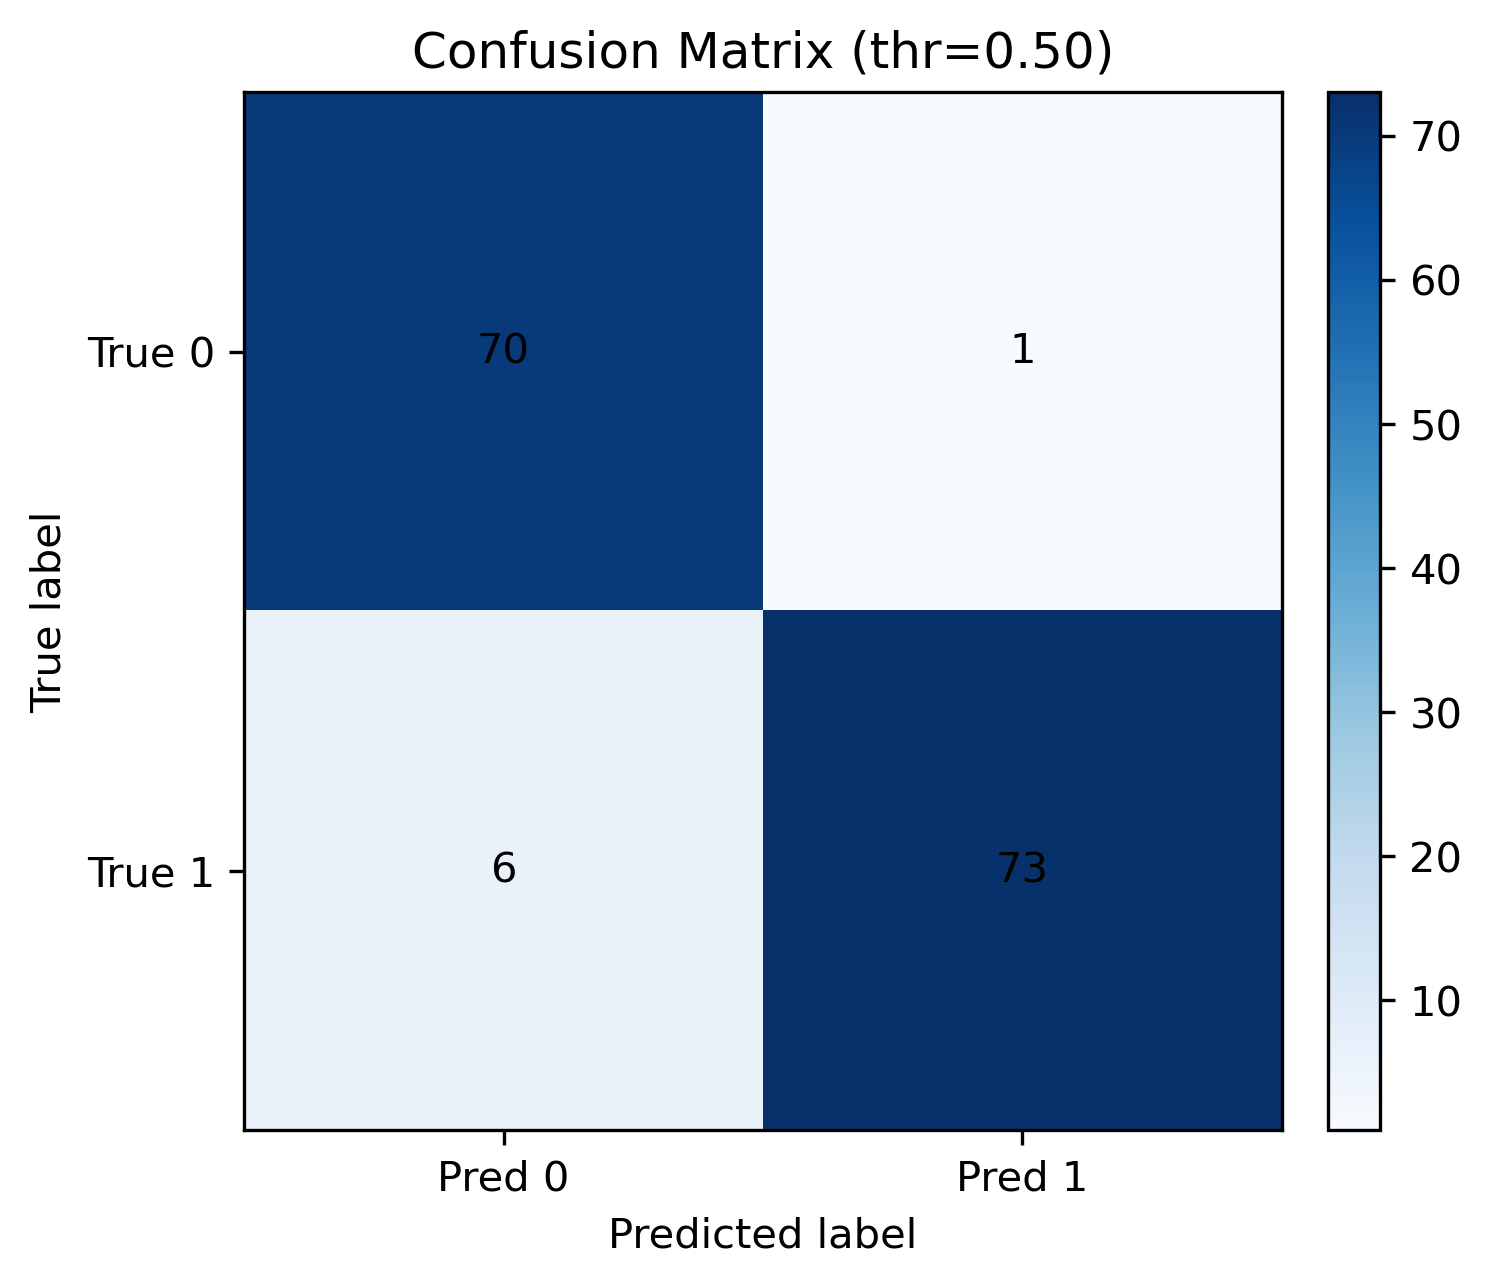
\includegraphics[width=0.6\linewidth]{confusion_matrix.png}
  \caption{在留出集上(阈值 0.5)的混淆矩阵}
  \label{fig:confusion}
\end{figure}

\FloatBarrier

\section{小结}
逻辑回归以简洁、可解释和高效著称,是分类任务中实用的基线模型。其概率化建模、凸优化训练和线性判别边界使之在工程与研究中长期占据重要地位。

\end{document}
